\chapter {The Homology module}

This\index{Homology groups!functions for computing} chapter is devoted to the description of the functions for
computing the homology groups of a chain complex.

\section {List of functions}

{\parindent=0mm
{\leftskip=5mm
{\tt chcm-homology} {\em chcm dim} \hfill {\em [Function]} \par}
{\leftskip=15mm
Return a description  of the homology group in dimension {\em dim} of the chain complex {\em chcm}
in terms of {\em components} of the form ${\Z}$ or ${\Z}/{n\, {\Z}}$. 
The desired homology group is the direct sum of these 
components. No canonical presentation is looked for, so that, if for instance, 
a homology group is ${\Z}/{6\, {\Z}}$, it can be displayed as one component
${\Z}/{6\, {\Z}}$ or two components ${\Z}/{2\, {\Z}}$ and ${\Z}/{3\, {\Z}}$.
On the other hand, if the component part  is void, this  means  the homology 
group is the null group. The function {\tt chcm-homology} implements the
usual algorithms to compute the homology group associated to two integer matrices,
the composite of which is null. The current version is verbose: for each group asked for,
the program displays the rank of each integer matrix and each generator of the source
module. Timing indications are also given. In the examples, only the  components are printed.
\par }
{\leftskip=5mm 
{\tt chcm-homology-gen} {\em chcm n} \hfill {\em [Function]} \par}
{\leftskip=15mm 
This function computes the homology group in dimension $n$ of the chain complex
{\em chcm} and prints a generator of degree $n$ in {\em chcm} for each component of 
the group (in general a combination of the  basis elements of degree $n$ of the
chain complex).\par}
{\leftskip=5mm 
{\tt chcm-mat} {\em chcm n} \hfill {\em [Function]} \par}
{\leftskip=15mm 
Return the   the  matrix of the li\-ne\-ar homomorphism 
$d_n: C_n \rightarrow C_{n-1}$, where
$C_n$ is the $n$--th chain group   of the chain complex  {\em chcm}. More precisely,
each column  of this matrix contains the integer coefficients in the basis of $C_{n-1}$ of 
the image by $d_n$ of each basis element of $C_n$. So the number of lines (resp. columns) of the matrix is
the number of elements of the basis of $C_{n-1}$ (resp. $C_n$).
The homology group
${\cal H}_n={\cal Z}_n/{\cal B}_n$ is computed from the two matrices 
{\tt MZ} $=$ {\tt chcm-mat {\em (chcm,n)}} and 
{\tt NB} $=$ {\tt chcm-mat {\em (chcm, n+1)}}. By well known algorithms 
on matrix reduction\footnote{{\bf S. MacLane \& G. Birkhoff}, {\em Algebra}, 
The MacMillan Company, 1967}, the matrix {\tt MZ}  is used
to find a basis for the kernel ${\cal Z}_n$ and the matrix {\tt NB}, to find in ${\cal Z}_n$ a presentation
of the group ${\cal H}_n={\cal Z}_n/{\cal B}_n$ by generators and relations. This is performed
by the internal function {\tt homologie} (beware: not {\tt homology}!).\par}
{\leftskip=5mm 
{\tt homology} {\em chcm  degr1 {\tt \&optional} (degr2 (1+ degr1))} \hfill {\em [Method]} \par}
{\leftskip=15mm 
Compute the homology groups from $degr_1$ to $degr_2-1$ (default: only $degr_1$, if {\em degr2} is omitted) of
the right chain complex of the homotopy equivalence contained in the slot {\tt :efhm} of the
chain complex instance {\em chcm}. At the creation of the chain complex, this slot is unbound and
is set during execution by an adequate CLOS method. If this slot cannot be  bound, an error is returned and
the homology groups cannot be computed. A more elaborated explanation of the mechanism used by the function
{\tt homology} is given in the  section: {\bf The general method for computing homology groups}. \par}
}

\subsection* {Example}

Let us get the homology groups for the example {\tt diabolo} of the chapter $1$.

{\footnotesize\begin{verbatim}
(chcm-homology diabolo 0)   ==>

Computing boundary-matrix in dimension 0.
Rank of the source-module : 6.
...

Homology in dimension 0 :

Component Z

(chcm-homology diabolo 1)   ==>

Computing boundary-matrix in dimension 1.
Rank of the source-module : 7.
...

Homology in dimension 1 :

Component Z

(chcm-homology diabolo 2)   ==>

Computing boundary-matrix in dimension 2.
Rank of the source-module : 1.
...

Homology in dimension 2 :

---done---
\end{verbatim}}
%\newpage
Another simple example is the following  2--chain  complex  corresponding to the
well known {\em dunce hat}. We shall see later in the chapter {\tt Simplicial Sets} a
much more elegant method to describe this object.
%
\vskip 0.40cm
\centerline{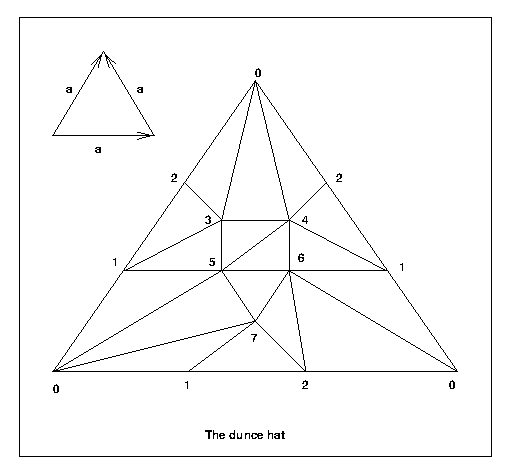
\includegraphics{dunce.eps}}
\vskip 0.40cm
%
The diagram shows a permissible triangulation. For the generators, we have  chosen lists 
rather symbols: a vertex $s_i$ is represented as {\tt (i)}, an edge $s_is_j$ as
{\tt (i j)} and a triangle $s_is_js_k$ as {\tt (i j k)}. The enumeration of
the elements of the basis is a little  cumbersome but defining  the
boundary homomorphism is very easy, bearing in mind the boundary rule:
$$ {\bf d}[s_0s_1\ldots s_n] = \sum_{i=0}^n{(-1)^is_0s_1\ldots\widehat{s_i}\ldots s_n}.$$
As for diabolo, the vertices are  implicitly ordered.
{\footnotesize\begin{verbatim}
  (setf duncehat-basis #'(lambda(dmn)
    (case dmn
       (0 '((0) (1) (2) (3) (4) (5) (6) (7) ))
       (1 '((0 1)(0 2)(0 3)
            (0 4)(0 5)(0 6)
            (0 7)(1 2)(1 3)
            (1 4)(1 5)(1 6)
            (1 7)(2 3)(2 4)
            (2 6)(2 7)(3 4)
            (3 5)(4 5)(4 6)
            (5 6)(5 7)(6 7) ))
       (2 '((0 1 5)(0 1 6)(0 1 7)
            (0 2 3)(0 2 4)(0 2 6)
            (0 3 4)(0 5 7)(1 2 3)
            (1 2 4)(1 2 7)(1 3 5)
            (1 4 6)(2 6 7)(3 4 5)
            (4 5 6)(5 6 7) ))
       (otherwise nil)) ))

  (setf duncehat-df #'(lambda(dmn gnr)
     (case dmn
        (0 (cmbn -1))
        (1 (cmbn 0  -1 (list(first gnr)) 1 (rest gnr)))
        (2 (cmbn 1 1 (list(first gnr) (second gnr))
                  -1 (list(first gnr) (third gnr))
                   1 (rest gnr) ))
        (otherwise (error "bad generator for dunce hat")))))


  (setf duncehat (build-chcm :cmpr #'l-cmpr
                             :basis duncehat-basis
                             :bsgn '(0)
                             :intr-dffr  duncehat-df
                             :strt :gnrt
                             :orgn '(dunce hat)))
\end{verbatim}}
\newpage
{\footnotesize\begin{verbatim}
(chcm-homology duncehat 0)   ==>

Computing boundary-matrix in dimension 0.
Rank of the source-module : 9.
...

Homology in dimension 0 :

Component Z

---done---

(chcm-homology duncehat 1)   ==>

Computing boundary-matrix in dimension 1.
Rank of the source-module : 27.
...

Homology in dimension 1 :

---done---

(chcm-homology duncehat 2)  ==>

Computing boundary-matrix in dimension 2.
Rank of the source-module : 19.
...

Homology in dimension 2 :

---done---
\end{verbatim}}

Let us take again  the chain complex {\tt duncehat}.
The two matrices of the homomorphisms $d_1: C_1 \rightarrow C_0$ and
$d_2: C_2 \rightarrow C_1$ are obtained by calling {\tt chcm-mat}.
{\footnotesize\begin{verbatim}
(setf mz (chcm-mat duncehat 1))  ==>

========== MATRIX 8 lines + 24 columns =====
L1=[C1=-1][C2=-1][C3=-1][C4=-1][C5=-1][C6=-1][C7=-1]
L2=[C1=1][C8=-1][C9=-1][C10=-1][C11=-1][C12=-1][C13=-1]
L3=[C2=1][C8=1][C14=-1][C15=-1][C16=-1][C17=-1]
L4=[C3=1][C9=1][C14=1][C18=-1][C19=-1]
L5=[C4=1][C10=1][C15=1][C18=1][C20=-1][C21=-1]
L6=[C5=1][C11=1][C19=1][C20=1][C22=-1][C23=-1]
L7=[C6=1][C12=1][C16=1][C21=1][C22=1][C24=-1]
L8=[C7=1][C13=1][C17=1][C23=1][C24=1]
========== END-MATRIX
\end{verbatim}}
\newpage
{\footnotesize\begin{verbatim}
(setf nb (chcm-mat duncehat 2))  ==>

========== MATRIX 24 lines + 17 columns =====
L1=[C1=1][C2=1][C3=1]
L2=[C4=1][C5=1][C6=1]
L3=[C4=-1][C7=1]
L4=[C5=-1][C7=-1]
L5=[C1=-1][C8=1]
L6=[C2=-1][C6=-1]
L7=[C3=-1][C8=-1]
L8=[C9=1][C10=1][C11=1]
L9=[C9=-1][C12=1]
L10=[C10=-1][C13=1]
L11=[C1=1][C12=-1]
L12=[C2=1][C13=-1]
L13=[C3=1][C11=-1]
L14=[C4=1][C9=1]
L15=[C5=1][C10=1]
L16=[C6=1][C14=1]
L17=[C11=1][C14=-1]
L18=[C7=1][C15=1]
L19=[C12=1][C15=-1]
L20=[C15=1][C16=1]
L21=[C13=1][C16=-1]
L22=[C16=1][C17=1]
L23=[C8=1][C17=-1]
L24=[C14=1][C17=1]
========== END-MATRIX

(homologie mz nb)  ==>

NIL
\end{verbatim}}
\newpage

\section {The general method for computing homology}

Among\index{Homology groups!general method in {\tt Kenzo}} the slots of the instance of an  object 
inheriting the {\tt CHAIN COMPLEX} class, a slot {\tt efhm}
has been reserved to point (possibly) to a homotopy e\-qui\-va\-len\-ce where the right bottom
chain complex is effective. The function {\tt homology} is designed to get
the right bottom chain complex of the homotopy equivalence value of the slot. If the
slot has been bound, then the homology groups are computed by the function {\tt chcm-homology}
as shown in the following de\-fi\-ni\-ti\-on:
{\footnotesize\begin{verbatim}
(DEFMETHOD HOMOLOGY ((chcm chain-complex) degr1 &optional (degr2 (1+ degr1)))
   (do ((degr degr1 (1+ degr)))
       ((>= degr degr2))
 -->   (chcm-homology (rbcc (efhm chcm)) degr)
       (terpri) (clock) (terpri)))
\end{verbatim}}
But, at the creation of the object, the slot {\tt efhm} is  unbound and as soon as the {\tt homology}
function tries to get the content of the slot {\tt efhm} via the call {\tt (efchm chcm)}, the
{\em slot-unbound} mechanism of CLOS is triggered, calling at its turn a method
{\tt search-efhm} depending on the object. If no method is available for this object,
{\tt NIL} is returned. In the following chapters, we shall see that cases have been
written for cartesian products, tensor products, suspensions, disk pasting, fibrations, 
loop spaces, and classifying spaces. The selection of the case is done thanks to the information 
contained in the comment list of the object (slot {\tt orgn}).
In each case,  the {\tt search-efhm} method builds -- in general with a complex machinery, including a possible
recursivity --
a homotopy equivalence where the right bottom
chain complex is {\em effective}. The slot {\tt efhm} of the object is then settled and the homology group
computation may begin. If {\tt NIL} is returned, then  and only at this moment, the slot-unbound
mechanism looks if the chain complex is finite (checking if a basis function exists). If this is the case, then
the {\em trivial homotopy equivalence} is built upon the chain complex and this gives the value of the slot
{\tt efhm}. If there is no basis function,  meaning that probably the chain complex is locally
effective, an error is returned.
\par
{\bf Remark.} The user may wonder why one does not  look first if the given object is effective.
We recall simply that even in the case of an effective chain complex, it is sometimes
possible to find another effective chain complex, homotopic to the first and whose 
number of basis elements, in any dimensions, is considerably smaller in comparison with the first one.
A striking case will be shown in a further chapter, showing the application of the
Eilenberg-Zilber theorem to a cartesian product.

\subsection*{Example}

{\bf The reading of this subsection may be postponed until a full reading of this user's guide}.
The following examples  show how are 
filled the slots {\tt efhm} of the various objects.
Starting from the sphere $S^2$, we  verify first that the {\tt efhm} slot is unbound.
Then we ask for ${\cal H}_1$ and verify that, though there is a finite basis,
{\tt Kenzo} has nevertheless built a trivial homotopy equivalence on this object. 
{\footnotesize\begin{verbatim}
(setf s2 (sphere 2))  ==>

[K1 Simplicial-Set]

(inspect s2)  ==>

SIMPLICIAL-SET @ #x39a1e2 = [K1 Simplicial-Set]
   0 Class --------> #<STANDARD-CLASS SIMPLICIAL-SET>
   1 ORGN ---------> (SPHERE 2), a proper list with 2 elements
   2 IDNM ---------> fixnum 1 [#x00000004]
-->3 EFHM ---------> The symbol :--UNBOUND--
   4 GRMD ---------> [K1 Simplicial-Set]
   5 DFFR ---------> [K2 Morphism (degree -1)]
   6 BSGN ---------> The symbol *
-->7 BASIS --------> #<Closure (FLET SPHERE-BASIS RSLT) @ #x39a14a>
   8 CMPR ---------> #<Function SPHERE-CMPR>
   9 CPRD ---------> [K5 Morphism (degree 0)]
  10 FACE ---------> #<Closure (FLET SPHERE-FACE RSLT) @ #x39a172>

(homology s2 1)  ==>

Homology in dimension 1 :

---done---

(inspect s2)  ==>

SIMPLICIAL-SET @ #x410372 = [K1 Simplicial-Set]

   .........................

-->3 EFHM ---------> [K9 Homotopy-Equivalence]

   ........................

(orgn (hmeq 9))  ==>

(TRIVIAL-HMEQ [K1 Simplicial-Set])
\end{verbatim}}
Now, we create $\Omega^1(S^2)$. Getting  the value of the slot {\tt efhm}
by a call to the accessor function {\tt efhm}, triggers the
search-efhm method for a loop space. A homotopy equivalence is built and
the slot is set.
{\footnotesize\begin{verbatim}
(setf os2 (loop-space s2))  ==>

[K10 Simplicial-Group]

(inspect os2)  ==>

SIMPLICIAL-GROUP @ #x4a208a = [K10 Simplicial-Group]

   ........................

-->3 EFHM ---------> The symbol :--UNBOUND--

   ........................

(orgn os2)  ==>

(LOOP-SPACE [K1 Simplicial-Set])

(efhm os2)  ==>

[K118 Homotopy-Equivalence]

(inspect os2)  ==>

SIMPLICIAL-GROUP @ #x30943a = [K10 Simplicial-Group]

   ...........................

   3 EFHM ---------> [K118 Homotopy-Equivalence]

   ...........................
\end{verbatim}}
The following example shows the recursion mechanism when one wants to get the value
of the slot {\tt efhm} of an iterated loop space, namely $\Omega^3(S^4)$.
{\footnotesize\begin{verbatim}

(setf s4 (sphere 4))  ==>

[K119 Simplicial-Set]

(inspect s4)  ==>

SIMPLICIAL-SET @ #x38647a = [K119 Simplicial-Set]

   ...........................

   3 EFHM ---------> The symbol :--UNBOUND--

   ...........................

(setf ooos4 (loop-space (loop-space (loop-space s4))))  ==> 

[K148 Simplicial-Group]

(orgn ooos4)  ==>

(LOOP-SPACE [K136 Simplicial-Group])

(orgn (second *))  ==>

(LOOP-SPACE [K124 Simplicial-Group])

(orgn (second *))  ==>

(LOOP-SPACE [K119 Simplicial-Set])

(orgn (second *))  ==>

(SPHERE 4)

(inspect (smgr 136))  ==>

SIMPLICIAL-GROUP @ #x463312 = [K136 Simplicial-Group]

   ............................

   3 EFHM ---------> The symbol :--UNBOUND--

   ............................

(inspect (smgr 124))  ==>

SIMPLICIAL-GROUP @ #x460efa = [K124 Simplicial-Group]

   ............................

   3 EFHM ---------> The symbol :--UNBOUND--

   ............................

(inspect (smst 119))  ==>

SIMPLICIAL-SET @ #x4102fa = [K119 Simplicial-Set]
   0 Class --------> #<STANDARD-CLASS SIMPLICIAL-SET>
   1 ORGN ---------> (SPHERE 4), a proper list with 2 elements

   ............................

   3 EFHM ---------> The symbol :--UNBOUND--

   ............................

(efhm ooos4)  ==>

[K522 Homotopy-Equivalence]

(inspect (smgr 136))  ==>

SIMPLICIAL-GROUP @ #x410e62 = [K136 Simplicial-Group]

   ...........................

   3 EFHM ---------> [K474 Homotopy-Equivalence]

   ...........................

(inspect (smgr 124))  ==>

SIMPLICIAL-GROUP @ #x41066a = [K124 Simplicial-Group]

   ...........................

   3 EFHM ---------> [K426 Homotopy-Equivalence]

   ...........................

(inspect (smst 119))  ==>

SIMPLICIAL-SET @ #x4191d2 = [K119 Simplicial-Set]

   ...........................

   3 EFHM ---------> [K412 Homotopy-Equivalence]

   ...........................

(inspect s4)  ==>

SIMPLICIAL-SET @ #x4191d2 = [K119 Simplicial-Set]

   ...........................

   3 EFHM ---------> [K412 Homotopy-Equivalence]

   ...........................

\end{verbatim}}



\subsection* {Lisp files concerned in this chapter}

{\tt homology-groups.lisp}, {\tt searching-homology}\par
and files containing a {\tt search-efhm} method.
